\documentclass{article}
\usepackage[utf8]{inputenc}
\parskip = 0.75em
\parindent = 10mm
\def\baselinestretch{1}
\usepackage {float}
\usepackage{listings}
\usepackage{subcaption}
\usepackage[usenames]{color}
\usepackage[numbers,sort&compress]{natbib}
\usepackage{multirow, array}
\usepackage[spanish]{babel}
	\deactivatetilden
	\spanishdecimal{.}
	\addto\captionsspanish{\def\tablename{Tabla}}
	\addto\captionsspanish{\def\listtablename{\'Indice de tablas}}

\usepackage{amsmath,amsfonts,amssymb}
	\allowdisplaybreaks[4]
\usepackage{graphicx}
	\graphicspath{{Figuras/}}
\usepackage[clearempty,pagestyles]{titlesec}
\usepackage{anysize}

\def\baselinestretch{1.5}
\papersize{27.9cm}{21.5cm} 
\marginsize{2cm}{2cm}{1cm}{1cm}

\begin{document}


	\begin{center}
	\huge{\textbf{Tarea 7 Búsqueda Local}}\\
	
	\textsc{ \Large Susana Ruiz Nuñez}
	\end{center}


\section{Planteamiento del problema} 
Para esta práctica se implementa una optimización heurística para encontrar máximos o mínimos locales de funciones \cite{satu}. En un primer momento se busca minimizar la función unidimensional, a partir de un punto seleccionado al azar, realizando movimientos locales. Se realizan n  réplicas, y el menor de ellos es el resultado de la búsqueda en sí.

\section{Metodología de trabajo}
Para lograr los objetivos de esta práctica se tuvo que cambiar la dirección del problema hacia maximización y además realizar la experimentación para dos dimensiones. La función inicial fue modificada como se muestra a continuación para fines de la práctica. 

\begin{equation}
	\label{eq:e1}
	g(x,y)= \frac{(x + 0.5)^4 - 25 * x^2 - 20 * x - 5 * x^2 + (y + 0.5)^4 - 30 * y^2 - 20 * y + 5 * y}{100} 
\end{equation}

Alcanzado el primer requisito de modificar ligeramente la función con la que se trabajaría a continuación, se prosiguió a cumplir con otros requisitos, tales como que la función fuera en dos dimensiones $g = (x, y)$ y para el rango comprendido entre $-3\leq x,y \leq 3$.
 
\begin{lstlisting}[language=R]
	low <- -3
	high <- 3
	step <- 0.01
	replicas <- 100
	replica <- function(t){
		curr <- c(runif(1, low, high))
		best <- curr
		for (tiempo in 1:t) {
			delta <- runif(1, 0, step)
			xl <- curr + c(-delta,0)
			xr <- curr + c(delta,0)
			yl <- curr + c(0,-delta)
			yr <- curr + c(0,delta)
			coordenadas <- c(xl,xr,yl,yr)
\end{lstlisting}

Lo siguiente a lograr era que la función objetivo alcanzara el máximo valor por lo que se planteó la relación de maximización.

\begin{lstlisting}[language=R]
	for(q in 1:4){
		val <- c(val, g(mejor1[q], mejor2[q]) )
	}
	maximo <- which.max(val)
	curr <- c(mejor1[maximo], mejor2[maximo])
	if(g(curr[1],curr[2]) > g(best[1],best[2])){ #Maximizar
		best <- curr
	}
	return(best)
\end{lstlisting}

\section{Resultados}
De los resultados obtenidos figura 1, se puede comentar la factibilidad del modelo para hallar el máximo local (ya que es un problema de maximización). Para pasos pequeños el modelo no nos da información valiosa, por lo que hay que proyectarlo para iteraciones más grandes. Se muestra como para 1000 pasos se va haciendo más evidente cuál es el valor objetivo de la función. Se puede observar también que no se obtienen en la iteraciones casi ningún valor disperso, por lo cual el modelo está demostrando su eficacia.   


\begin{figure}
	\centering
	\begin{subfigure}[b]{0.45\linewidth}
		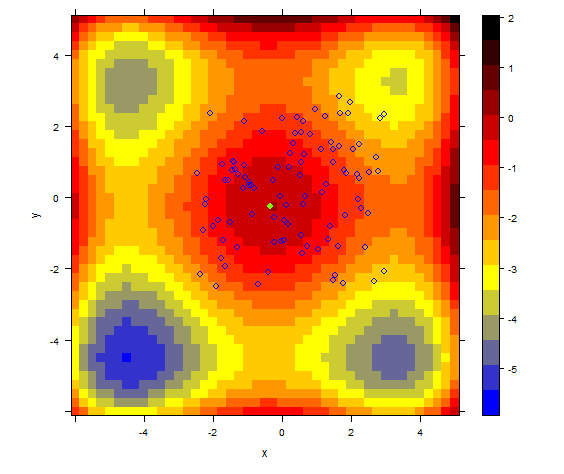
\includegraphics[width=\linewidth]{t7100.png}
		\caption{Experimento para 100 pasos.}
		\label{1}
	\end{subfigure}
		\begin{subfigure}[b]{0.45\linewidth}
		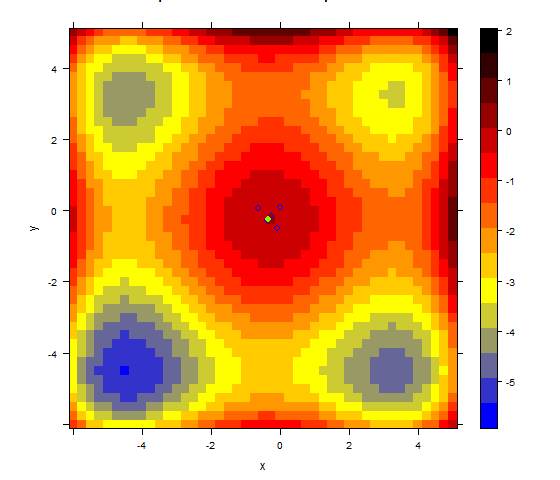
\includegraphics[width=\linewidth]{t71000.png}
		\caption{Experimento para 1000 pasos.}
		\label{2}
	\end{subfigure}
		\begin{subfigure}[b]{0.45\linewidth}
			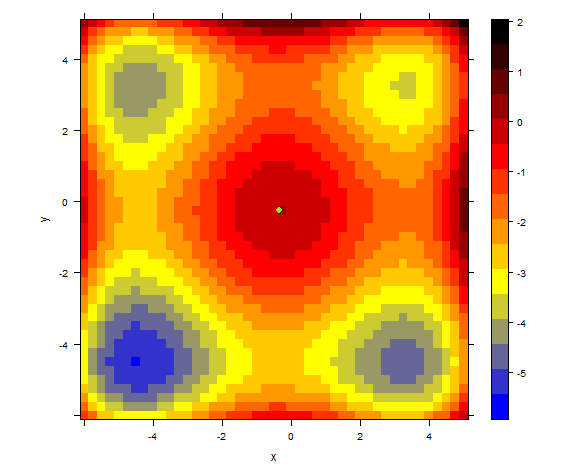
\includegraphics[width=\linewidth]{t710000.png}
			\caption{Experimento para 10000 pasos.}
			\label{3}
	\end{subfigure}
	\caption{Búsqueda Local para diferentes números de pasos.}  		
\end{figure}

\subsection{Resultados del gif}

Para la mejor comprensión de lo que sucede para distintos puntos figura 2, que están buscando el mejor valor de la función, se representó a través de un gif lo que ocurre para seis puntos que parten de diferentes posiciones. este experimento se realizó para un total de 100 iteraciones donde se ve como ya en la iteración 70 casi todos los puntos encontraron el mejor valor, lo que da validez al método utilizado. 

\begin{figure}[H]
	\centering
	\begin{subfigure}[b]{0.45\linewidth}
		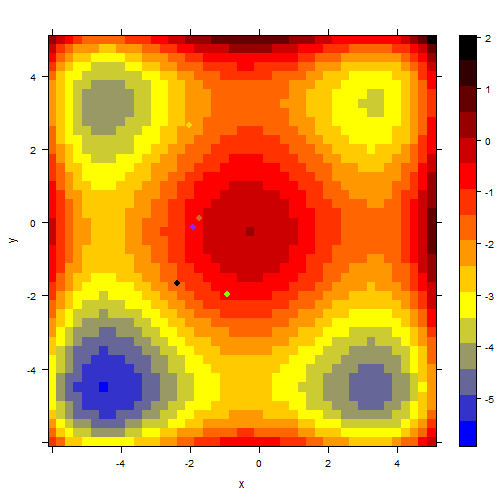
\includegraphics[width=\linewidth]{f1n001.png}
		\caption{Experimento en iteración 1.}
		\label{1}
	\end{subfigure}
	\begin{subfigure}[b]{0.45\linewidth}
		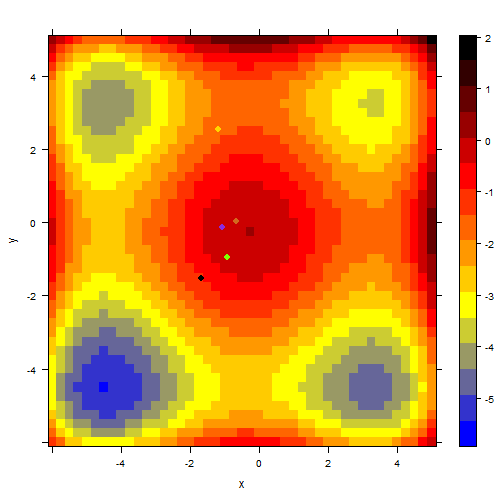
\includegraphics[width=\linewidth]{f1n020.png}
		\caption{Experimento en iteración 20.}
		\label{2}
	\end{subfigure}
	\begin{subfigure}[b]{0.45\linewidth}
		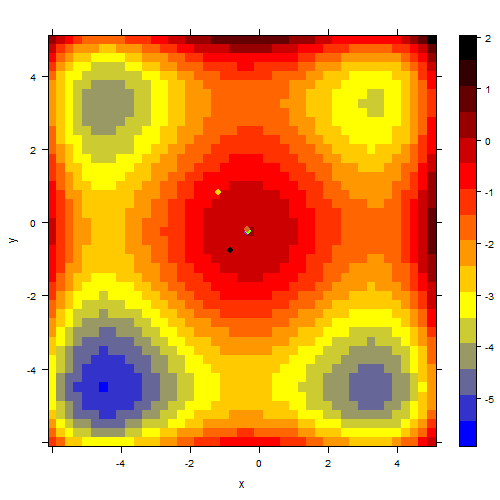
\includegraphics[width=\linewidth]{f1n050.png}
		\caption{Experimento en iteración 50.}
		\label{3}
	\end{subfigure}
	\begin{subfigure}[b]{0.45\linewidth}
		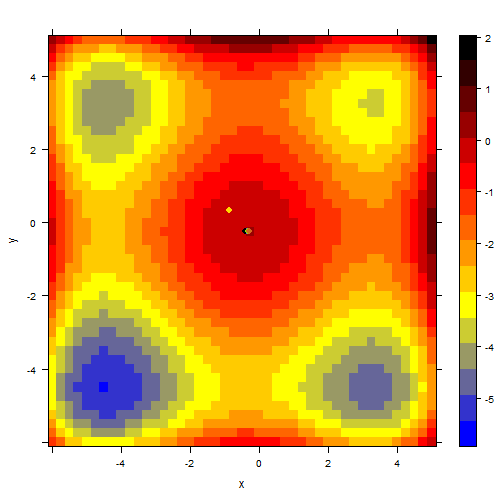
\includegraphics[width=\linewidth]{f1n070.png}
		\caption{Experimento en iteración 70.}
		\label{4}
	\end{subfigure}
	\caption{Muestra del gif para 6 réplicas simultáneas.}  		
\end{figure}

\section{Conclusiones}
Se concluye con los experimentos realizados que el método heurístico utilizado es bastante eficaz para la resolución de problemas donde se quiere hallar un máximo o mínimo local. En los resultados se muestra como la mayoría de las veces el modelo llegó al valor buscado.

\bibliography{Tarea7}
\bibliographystyle{plainnat}
\end{document} 
